\begin{figure*}[t]
    \setlength{\resLen}{1.5in}
    %
    \centering
    \small
    \addtolength{\tabcolsep}{-5.5pt}
    %
    %
    \begin{tabular}{cc}
        % &
        (a) \textbf{Forward} & (b) \textbf{Opacity Values Along the Ray}
        \\
        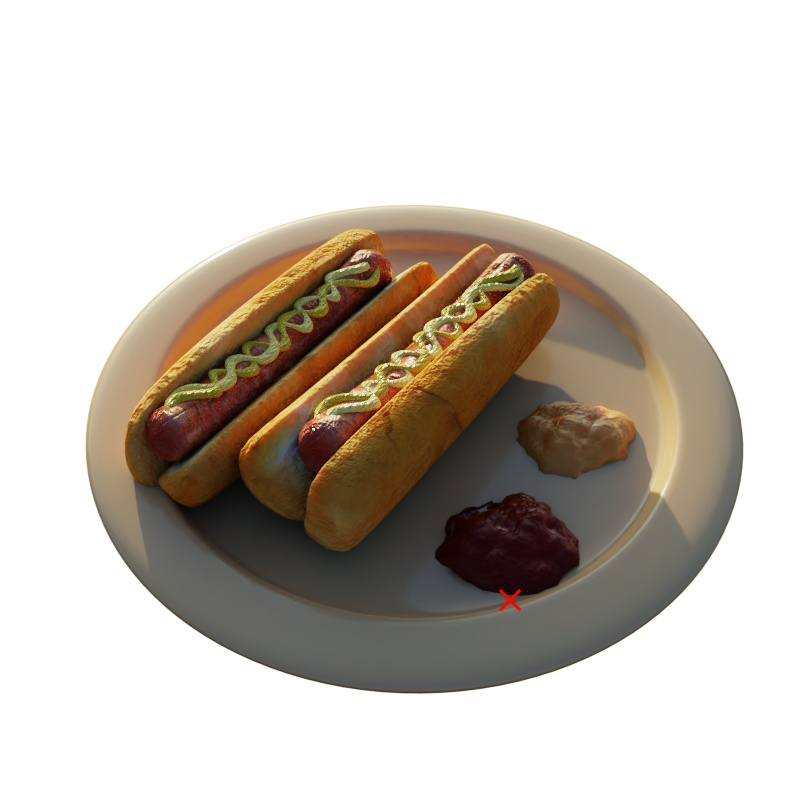
\includegraphics[trim={30 0 30 100}, clip, width=\resLen]{images/grad_image/forward_mark.jpg} &
        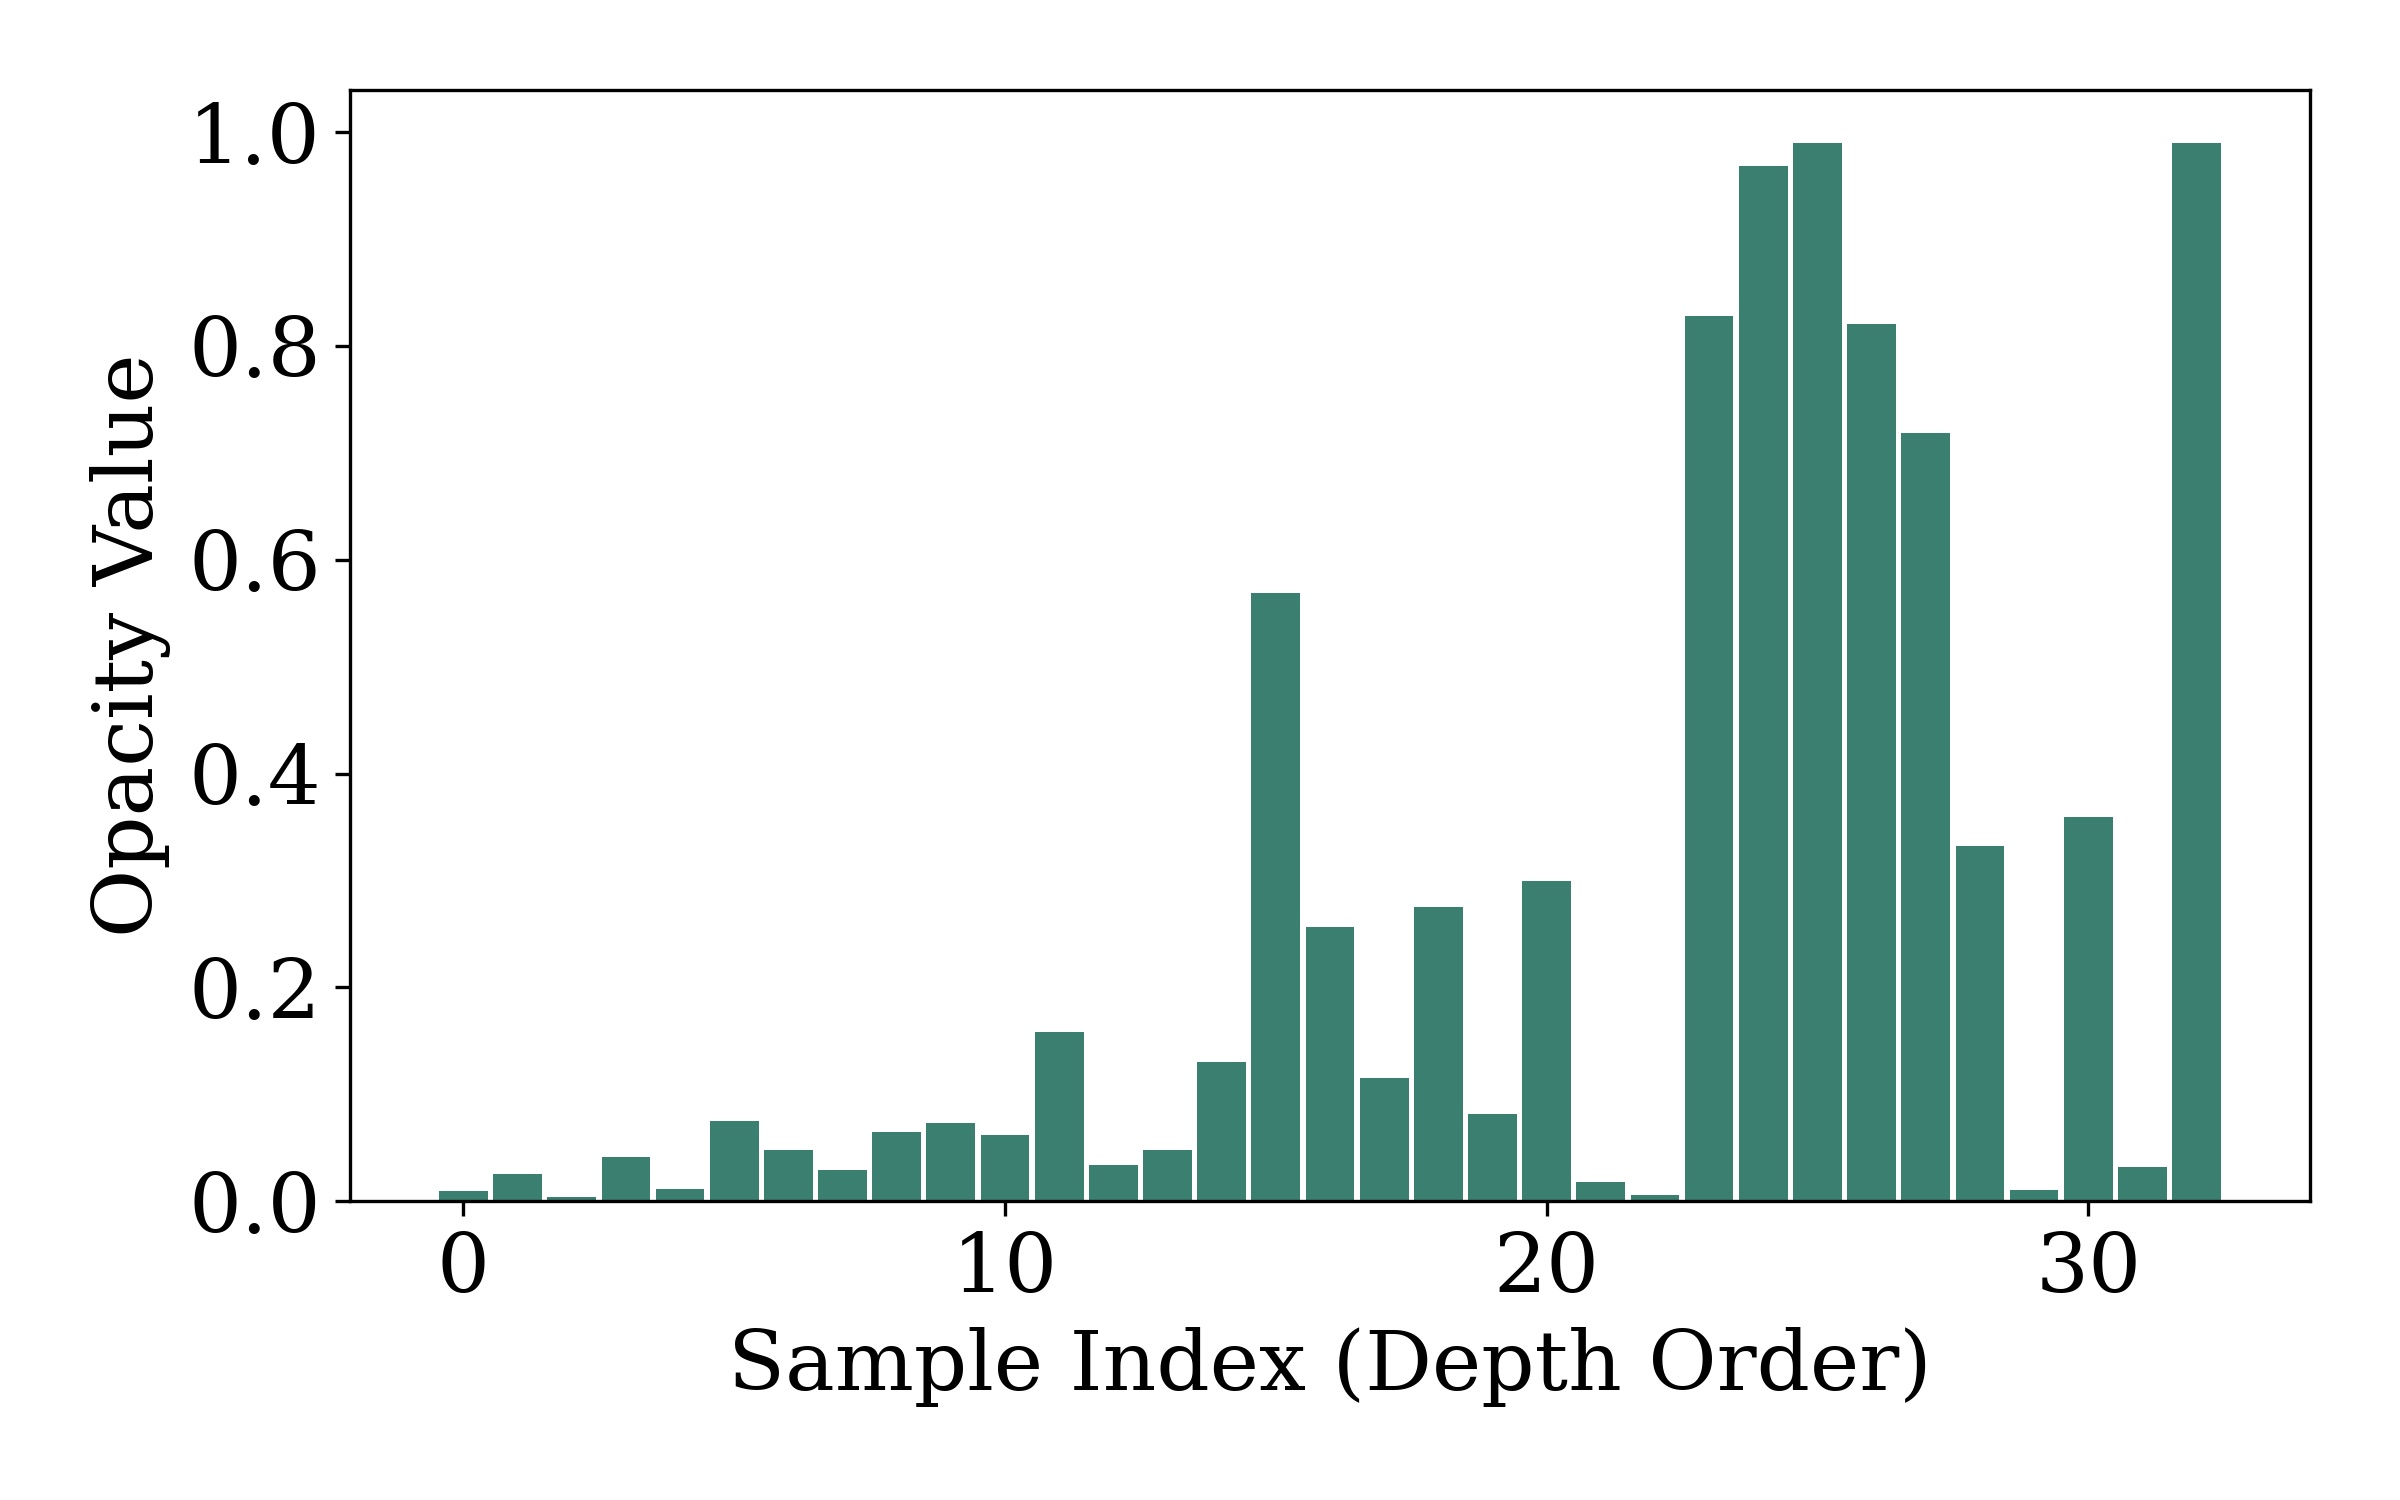
\includegraphics[height=\resLen]{images/grad_image/alpha_histogram.jpg}
    \end{tabular}
    \begin{tabular}{cccc}
        % &
        (c) \textbf{Sorted} & (d) \textbf{Ours, $M_b=8$}  & (e) \textbf{SS-Tracing, $M_b=8$}  & (f) \textbf{SS-Tracing, $M_b=128$}
        \\
        \begin{overpic}[trim={30 0 30 100}, clip, width=\resLen]{images/grad_image/AB.jpg}
            \put(50, 0){\makebox(0,0){\color{black}{\scriptsize \textbf{Time: 21.46ms}}}}
        \end{overpic} &
        \begin{overpic}[trim={30 0 30 100}, clip, width=\resLen]{images/grad_image/ours_8spp.jpg}
            \put(50, 0){\makebox(0,0){\color{black}{\scriptsize \textbf{Time: 10.87ms | RMSE: 0.408}}}}
        \end{overpic} &
        \begin{overpic}[trim={30 0 30 100}, clip, width=\resLen]{images/grad_image/ssplats_8spp.jpg}
            \put(50, 0){\makebox(0,0){\color{black}{\scriptsize \textbf{Time: 28.22ms | RMSE: 1.432}}}}
        \end{overpic} &
        \begin{overpic}[trim={30 0 30 100}, clip, width=\resLen]{images/grad_image/ssplats_128spp.jpg}
            \put(50, 0){\makebox(0,0){\color{black}{\scriptsize \textbf{Time: 484.04ms | RMSE: 0.427}}}}
        \end{overpic}
    \end{tabular}
    %
    \caption{
        Visualization of the variance of the gradient obtained by our method and the baseline method. (a) shows the forward rendering result, and (b) visualizes the opacities of each Gaussian along the ray at the red cross in (a). We further visualize the gradient that the Gaussians along each pixel receive when applying: (c) Sorted alpha blending (3DGRT), (d) Ours, with $M_b=8$, (e) Our implementation of~\cite{kv2025stochasticsplats}, with $M_b=8$, and (f) Our implementation of~\cite{kv2025stochasticsplats}, with $M_b=128$. The time for the backward pass and RMSE are provided with each image.
    }
    \label{fig:gradient_image}
\end{figure*}